\DailyTitle{6371 Log (November 22, 2010)}

\DailySection{Timing performance on \texttt{MultiJet} dataset}

Run on \texttt{MultiJet} dataset, as per suggestion from Maria.
10000 events, run 147754, file \texttt{D2B675A9-91D5-DF11-B6A2-0030487C6088.root}
Result is in the following plot \ref{Figure_6371_MultiJetExecutionTime}.

\begin{figure}[htbp]
   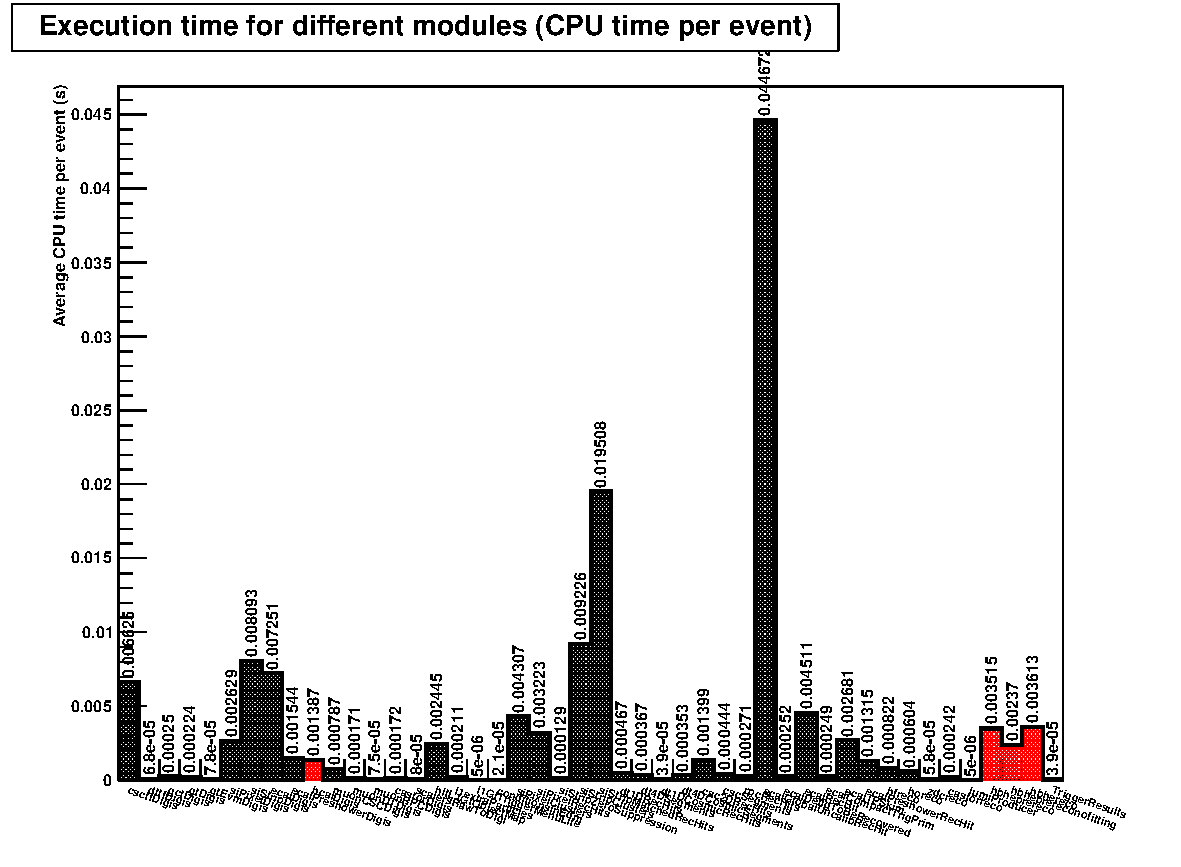
\includegraphics[width=120mm]{DailyLog/6371/6371_MultiJetExecutionTime}
   \caption{Average CPU time per event for \texttt{MultiJet} dataset, run 147754}
   \label{Figure_6371_MultiJetExecutionTime}
\end{figure}

\DailySection{Smoothing out cut positions}

Eye-balled cut positions.  Before/after are shown in figure \ref{Figure_6371_SmoothedCutPositions}.  The HBHE MET performance is OK.

\begin{figure}[htbp]
   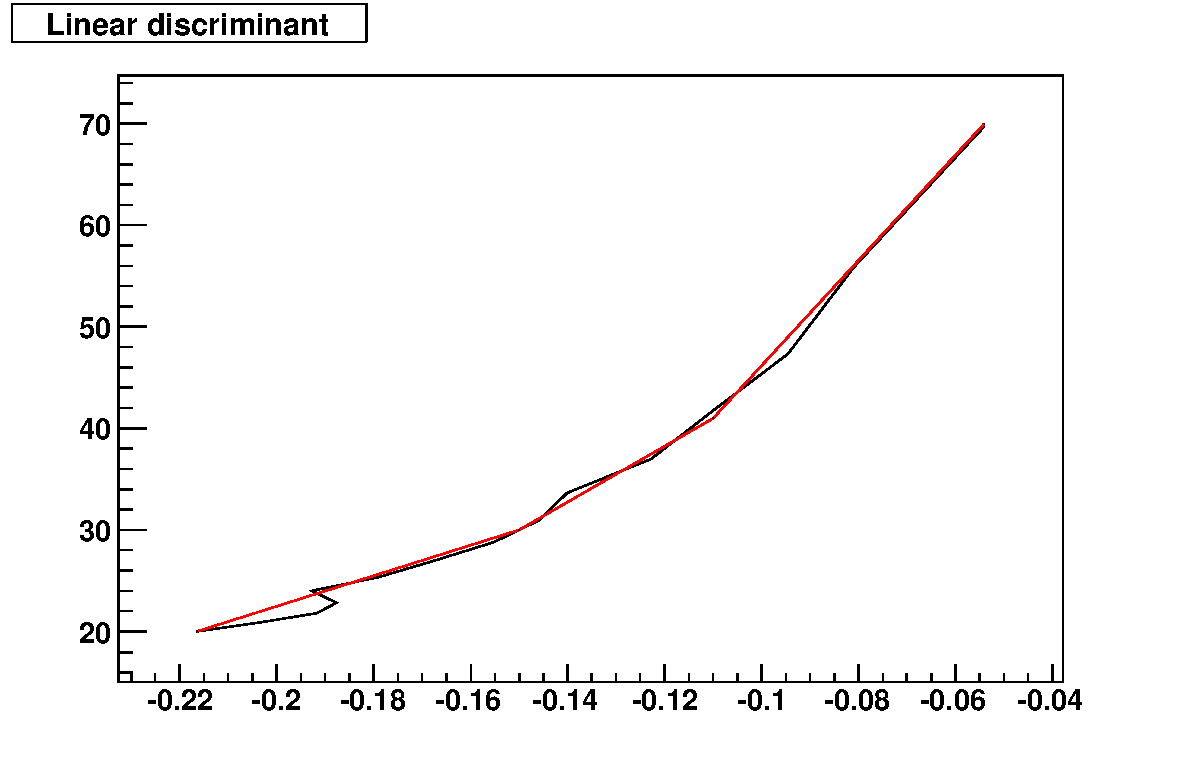
\includegraphics[width=60mm]{DailyLog/6371/6371_CutPosition_Linear}
   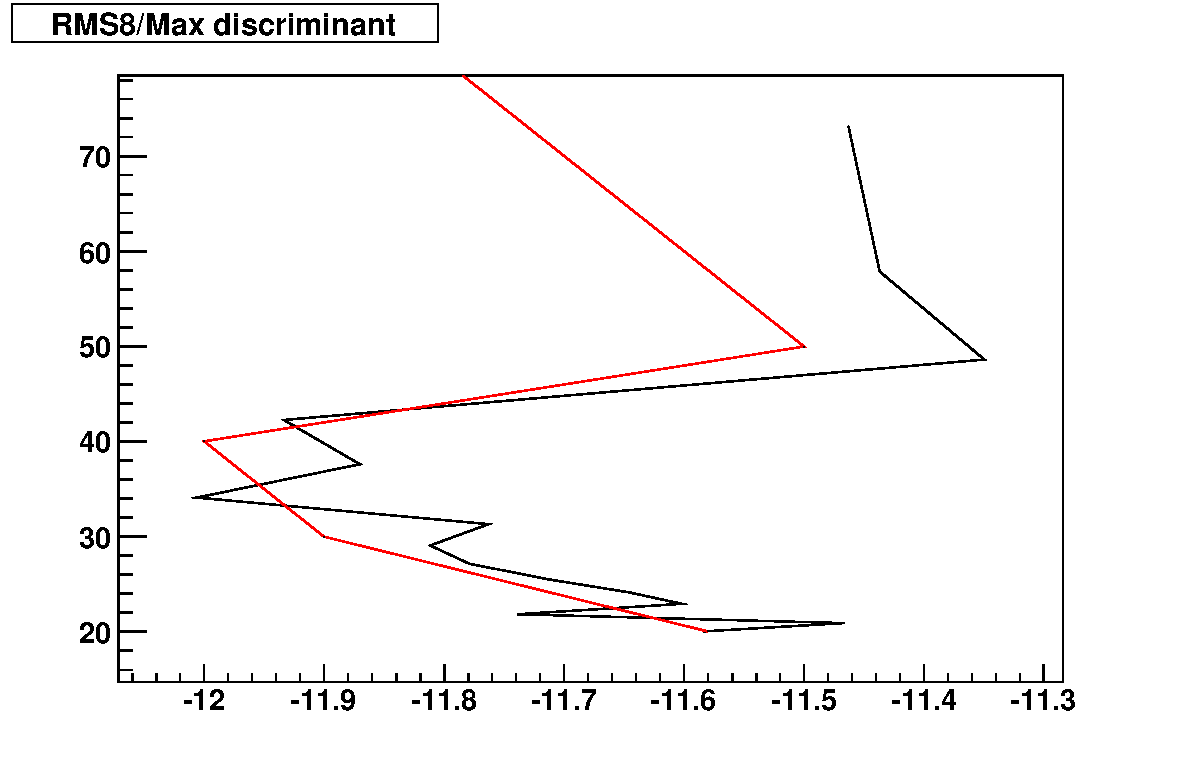
\includegraphics[width=60mm]{DailyLog/6371/6371_CutPosition_Spike}
   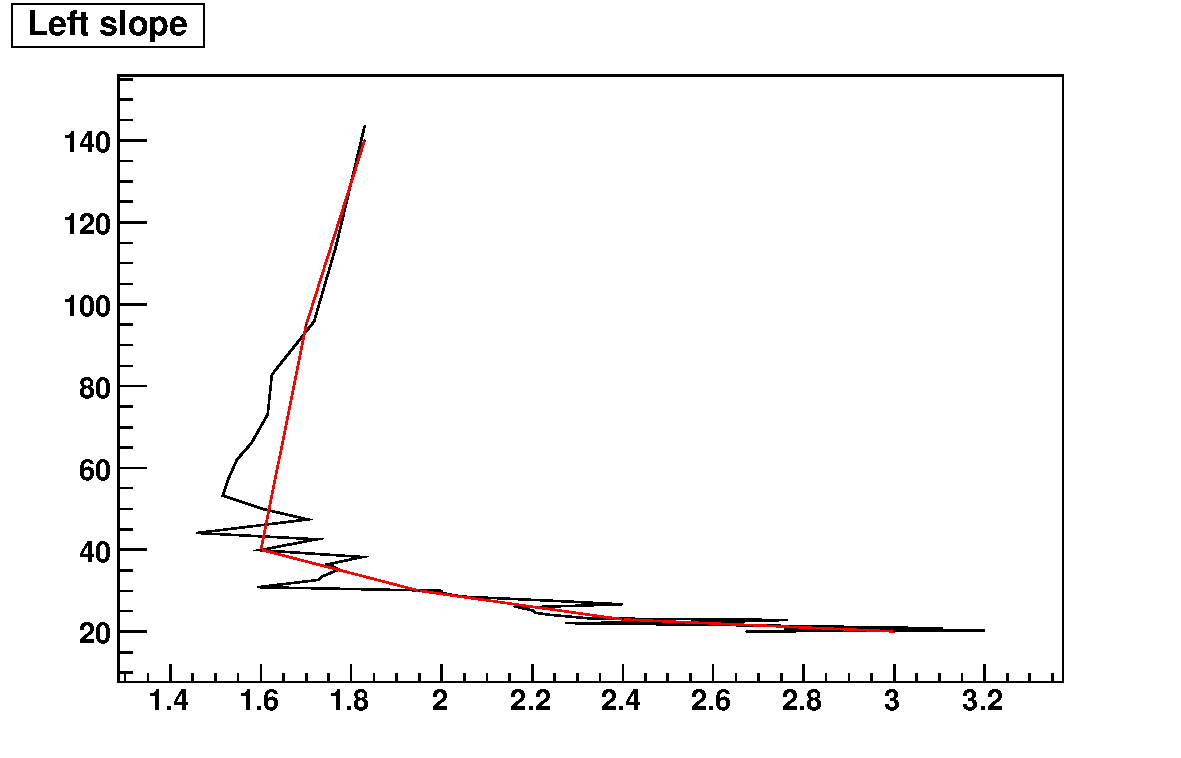
\includegraphics[width=60mm]{DailyLog/6371/6371_CutPosition_LeftSlope}
   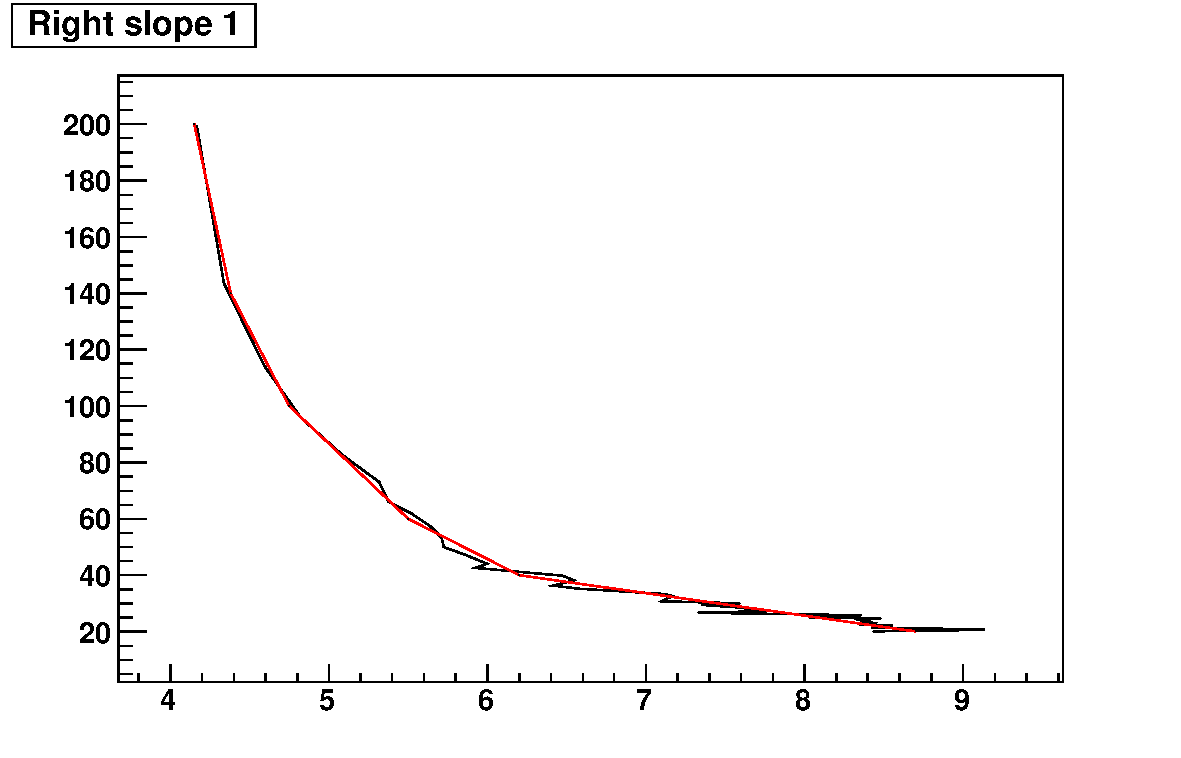
\includegraphics[width=60mm]{DailyLog/6371/6371_CutPosition_RightSlope1}
   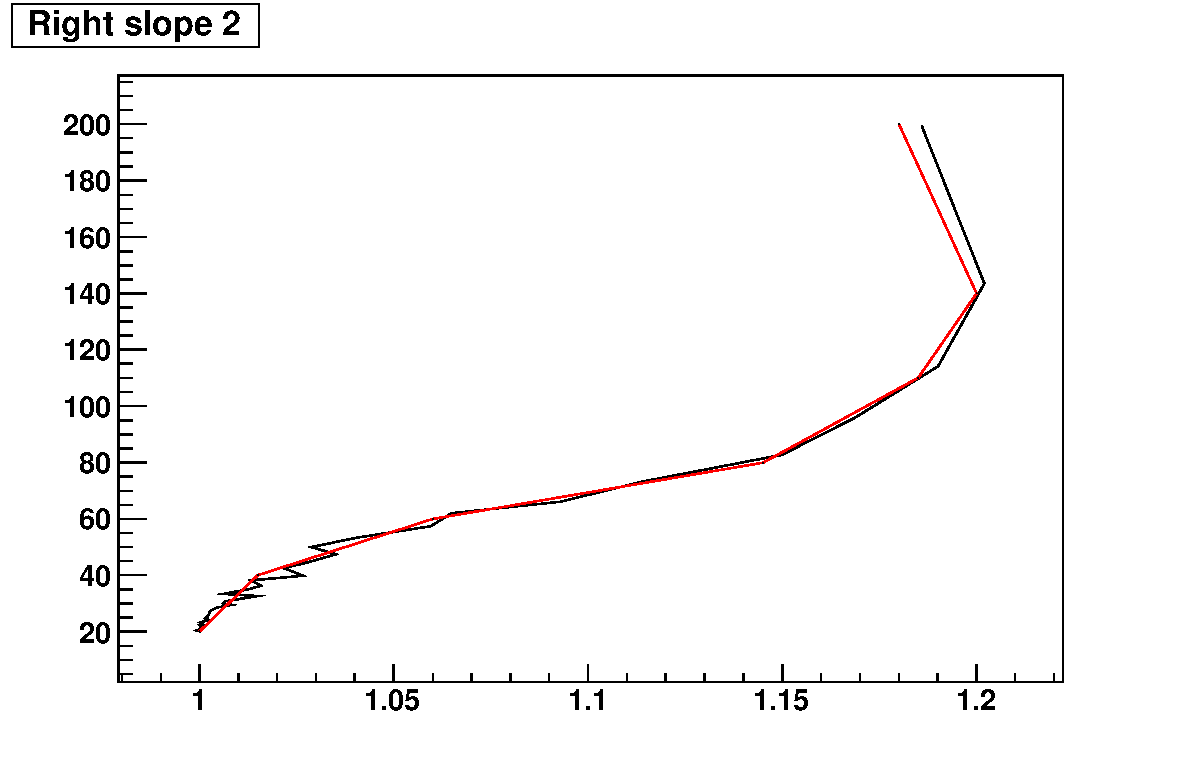
\includegraphics[width=60mm]{DailyLog/6371/6371_CutPosition_RightSlope2}
   \caption{Before (black) and after (red) smoothing cut positions.}
   \label{Figure_6371_SmoothedCutPositions}
\end{figure}

\DailySection{First look at run 149442}

Bunch crossing map is shown in figure \ref{Figure_6371_149442_BunchCrossings}.
All the groups are in 100 ns bunch spacing, except for the two groups around 1850 and 2240 (50 ns bunch spacing).
Looking at the average number of reconstructed primary vertex (roughly a measure of average pile-up),
the two groups with 50 ns bunch spacing have on average 1.7 pile-ups per event (figure \ref{Figure_6371_Run149442_50nsGroups_NumberOfGoodPrimaryVertices}).
Doing some back-of-the-envelope calculation, 11\% of MB events will have overlap of 10fC or more.
If we raise the threshold to 20fC, the overlap rate is 1.1\%.

Indeed there are evidence of late/early pileups.  See figure \ref{Figure_6371_EarlyLatePulses}.  Now what do I need to be looking at?
There is a perplexing thing that even in the non-50ns groups in run 149442 there seems to be pile-ups that are 50ns late.  Why?

\begin{figure}[htbp]
   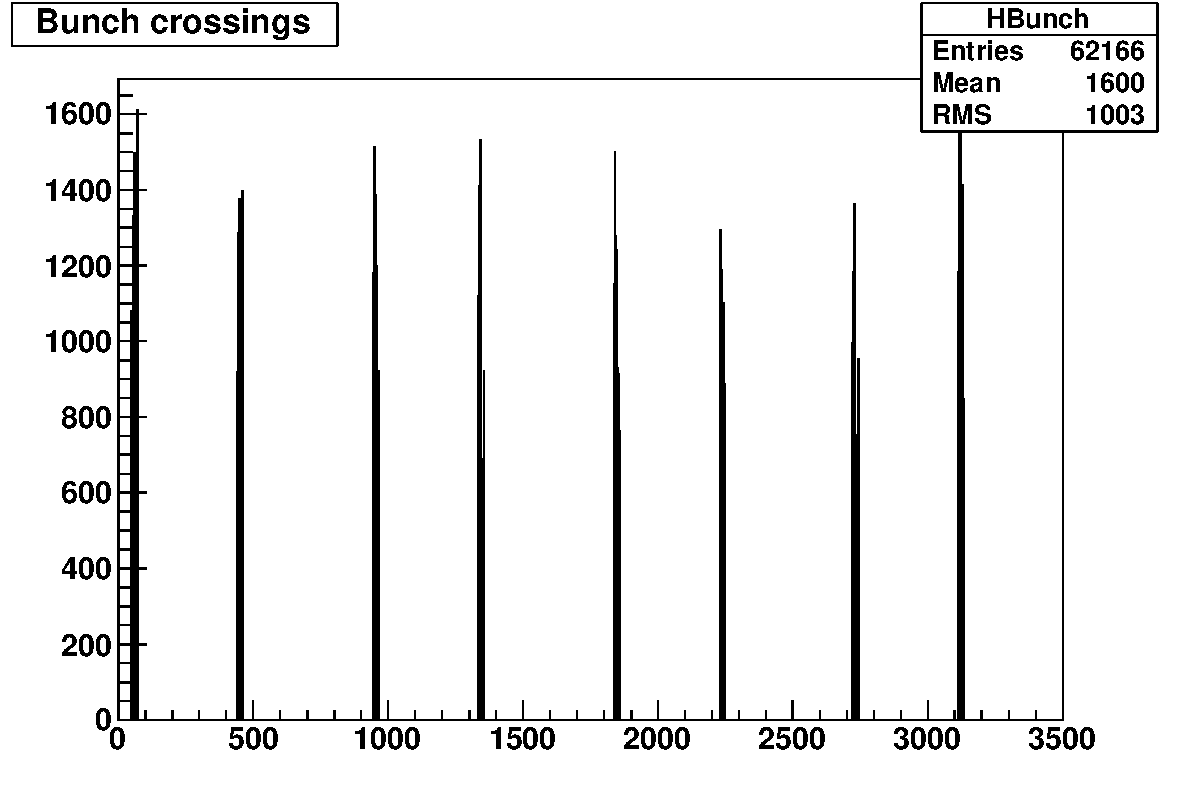
\includegraphics[width=120mm]{DailyLog/6371/6371_Run149442_Bunch}
   \caption{Bunch crossings fro run 149442 (\texttt{Jet} dataset).}
   \label{Figure_6371_149442_BunchCrossings}
\end{figure}

\begin{figure}[htbp]
   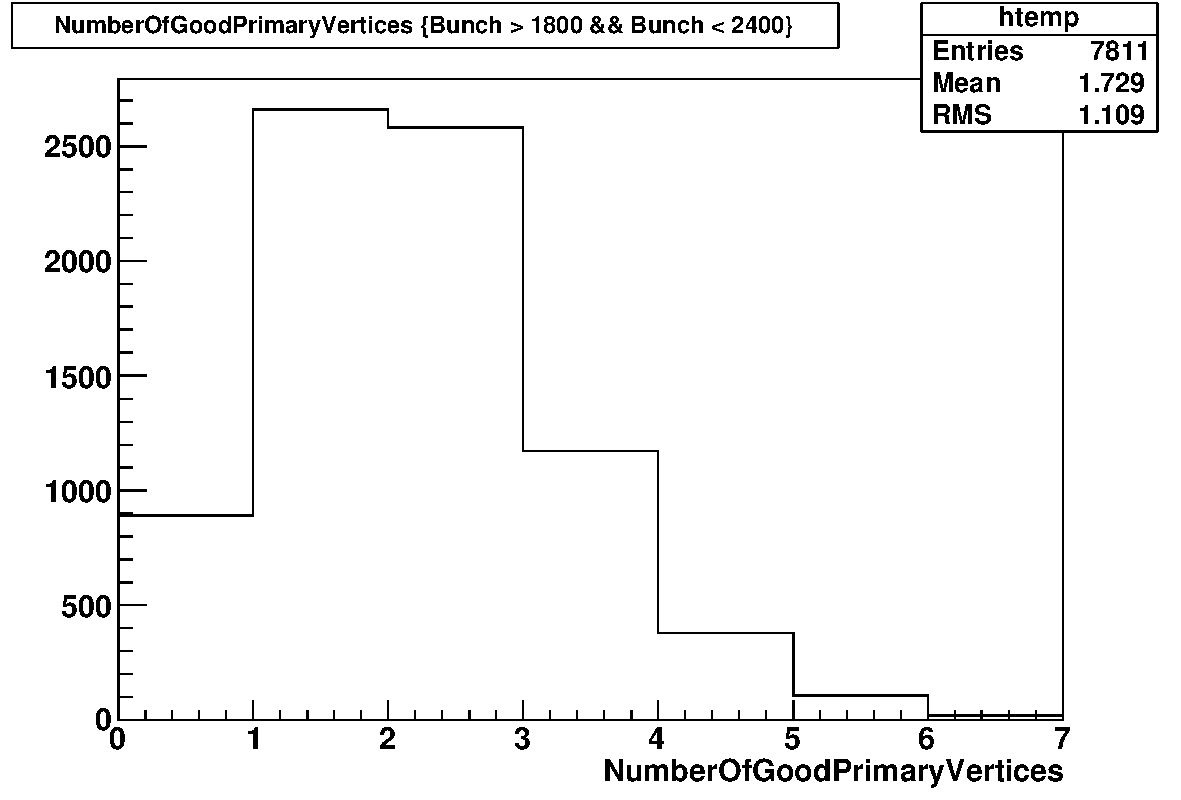
\includegraphics[width=120mm]{DailyLog/6371/6371_Run149442_50nsGroups_NumberOfGoodPrimaryVertices}
   \caption{Number of reconstructed good primary vertices for the 50ns spacing events.}
   \label{Figure_6371_Run149442_50nsGroups_NumberOfGoodPrimaryVertices}
\end{figure}

\begin{figure}[htbp]
   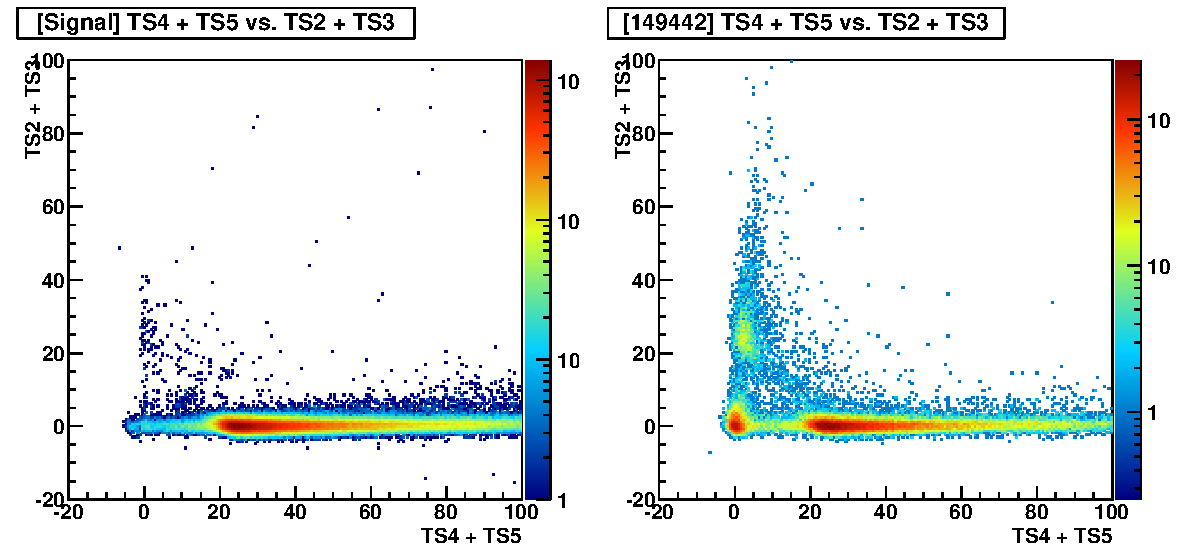
\includegraphics[width=120mm]{DailyLog/6371/6371_Comparison_HTS45VsTS23}
   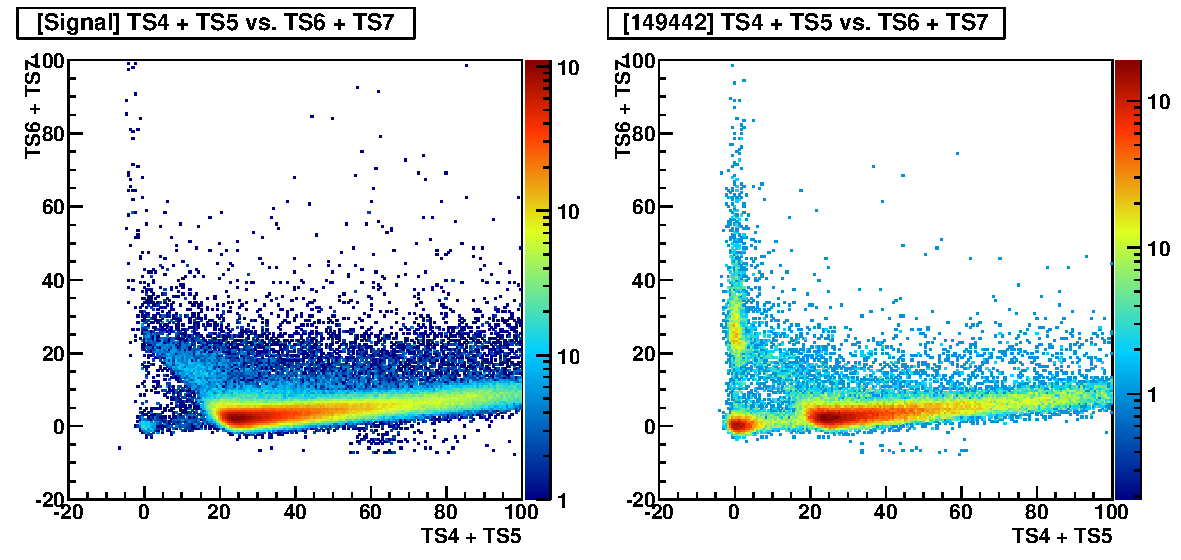
\includegraphics[width=120mm]{DailyLog/6371/6371_Comparison_HTS45VsTS67}
   \caption{Late/early pile up}
   \label{Figure_6371_EarlyLatePulses}
\end{figure}



